\section{Resultados}

A continuación incluiremos graficos comparativos cuyo objetivo es el de mostrar como funciona nuestro algoritmo en situaciones estándar y especiales que creemos merecen especial consideración. En todos los casos se usó un radio interior igual a 0.1 y un radio exterior igual a 1

\subsection{Comparación entre discretizaciones con diferentes cantidades de ángulos}

En este caso hicimos dos gráficos, para el primero establecimos la cantidad de ángulos fija en 10, y fuimos variando la cantidad de círculos de 20 en 20, desde 5 hasta 85. Las 10 temperaturas exteriores las generamos de manera aleatoria en una página de internet (Sección \ref{referencias}), obviamente teniendo en cuenta las restricciones que se aplican a las mismas.

\vspace{2cm}

\begin{center}
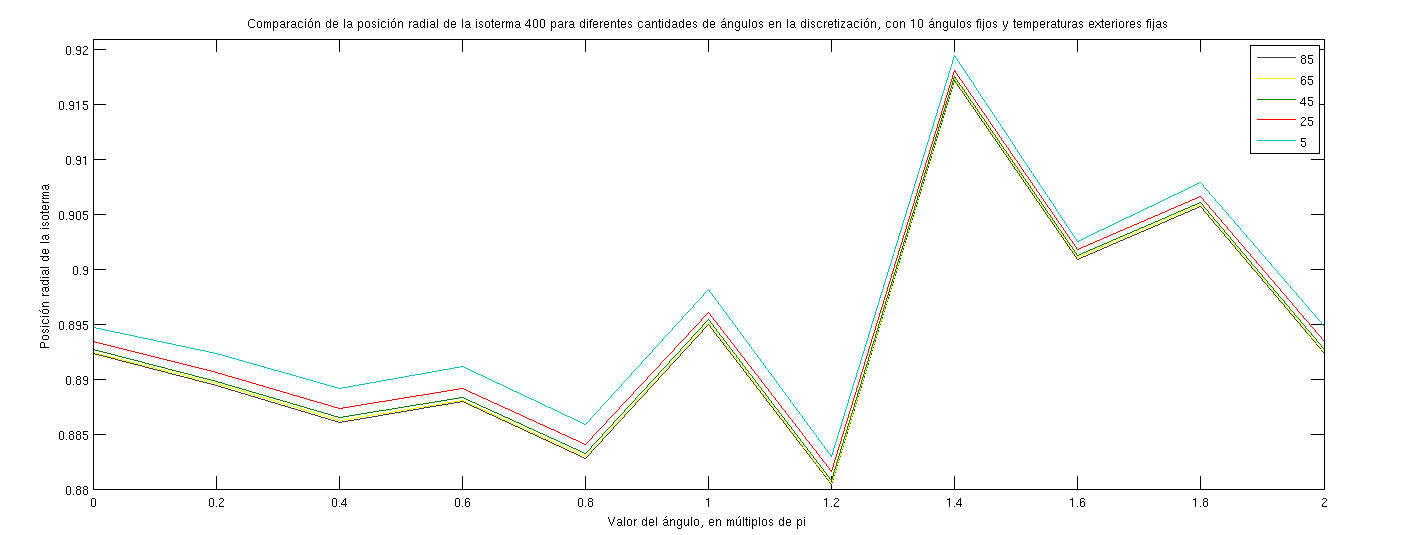
\includegraphics[scale=0.45]{../img/correccion-10ang.png}
\scriptsize{\textsf{\textbf{Gr\'afico 1.1, comparación de la posición radial de la isoterma de 400º para diferentes cantidades de ángulos en la discretización, con 10 ángulos fijos y temperaturas exteriores fijas aleatorias. El eje Y empieza en 0.88 porque no pudimos introducir un corte de escala en MATLAB}}}
\end{center}

\vspace{2cm}


Luego graficamos otro set de datos donde nuevamente dejamos la cantidad de ángulos fija, esta vez en 30, usando las mismas variaciones de cantidades de círculos que en el experimento anterior. Nuevamente, las temperaturas exteriores fueron generadas de manera aleatoria por \textit{random.org}

\vspace{2cm}

\begin{center}
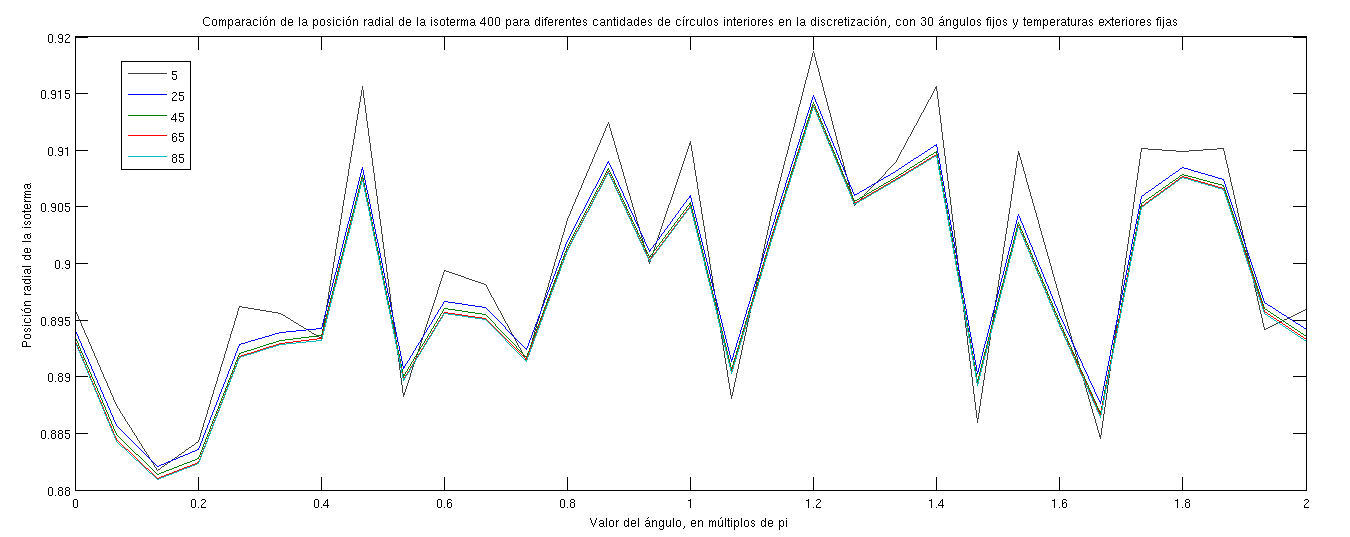
\includegraphics[scale=0.45]{../img/correccion-30ang.png}

\scriptsize{\textsf{\textbf{Gr\'afico 1.2, comparación de la posición radial de la isoterma de 400º para diferentes cantidades de ángulos en la discretización, con 30 ángulos fijos y temperaturas exteriores fijas aleatorias. El eje Y empieza en 0.88 porque no pudimos introducir un corte de escala en MATLAB}}}
\end{center}

\vspace{2cm}

\subsection{Caso especial}

Nos pareció interesante estudiar el comportamiento de nuestro programa en un caso especial, esto es, en el que temperaturas exteriores consecutivas alternan entre 50 y 200 constantemente. Esto lo comparamos con un set de temperaturas exteriores generado al azar por \textit{random.org}, pero con la restricción de que todas estuvieran entre 90 y 100, a manera de asegurar que la varianza sea menor a 10. En ambos casos se usaron 50 ángulos y 50 círculos.

\vspace{2cm}

\begin{center}
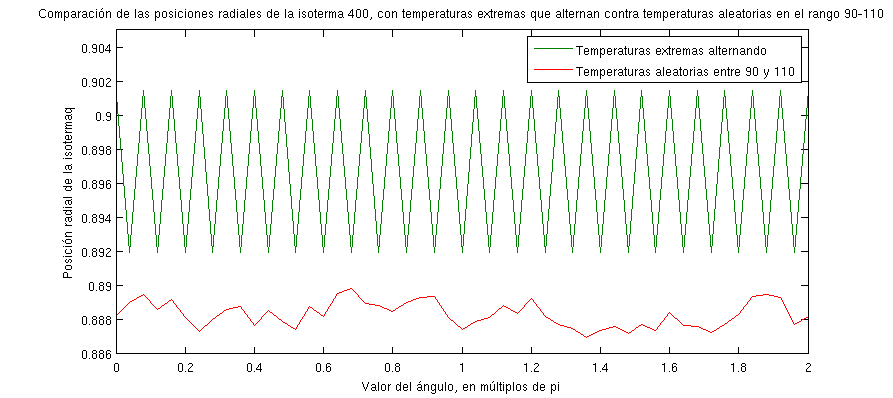
\includegraphics[scale=0.6]{../img/correccion-extremas.png}

\scriptsize{\textsf{\textbf{Gr\'afico 2.1, comparación de las posicionen radiales de la isoterma 400 con temperaturas extremas que alternan contra temperaturas aleatorias en el rango 90-100, en ambos casos usando 50 ángulos y 50 círculos. El eje Y empieza en 0.886 porque no pudimos introducir un corte de escala en MATLAB}}}
\end{center}
\vspace{2cm}

\subsection{Tiempo transcurrido}

Para este caso analizamos el tiempo que demora efectuar todos los cálculos para diferentes discretizaciones del problema. Para esto, empezamos con 5 ángulos y 5 círculos e incrementamos de 5 en 5 ambas cantidades (con lo cual el número de ecuaciones crece cuadráticamente), y usamos un set de temperaturas exteriores generado al azar por \textit{random.org} Ante cada entrada del programa usamos la función $time$ de UNIX y extrajimos el valor que nos devolvía del campo $real$ para hacer este gŕafico. Tratamos de que todas las corridas se llevaran a cabo en un entorno similar, con los mismos procesos corriendo, de manera tal que eso no afecte los resultados obtenidos

\vspace{2cm}

\begin{center}
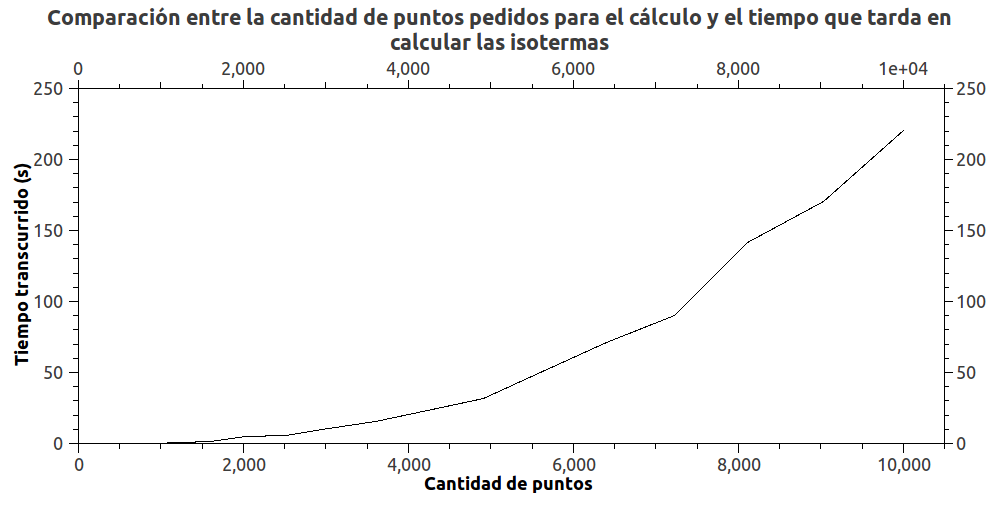
\includegraphics[scale=0.55]{../img/Grafico.png} \\
\scriptsize{\textsf{\textbf{Gr\'afico 3.1, Gráfico del tiempo insumido por el programa con diferentes cantidades de puntos a analizar}}}
\end{center}
%
%\vspace{2cm}
%
%\begin{center}
%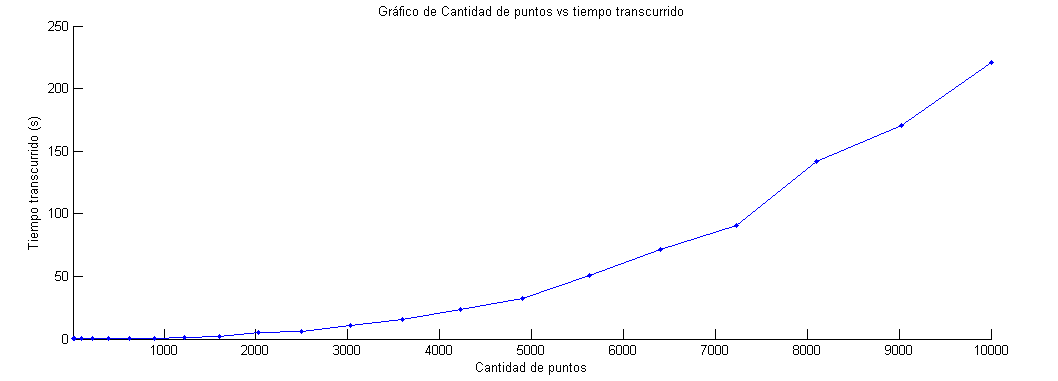
\includegraphics[scale=0.55]{../img/tiempoVsPuntos.png} \\
%\scriptsize{\textsf{\textbf{Gr\'afico 3.1, Gráfico del tiempo insumido por el programa con diferentes cantidades de puntos a analizar}}}
%\end{center}


